\section{Goal Description}

    \subsection{Problem}
      Within the UK, 49\% of adults own a pet. With around 25\% owning cats and 24\% owning dogs. This makes the total number of cats and dogs in the UK around 20 million. That’s a lot of pets to feed daily. What’s more, the UK loves it’s pets, with households routinely making pets a huge part of their family. This means that when away on holiday, or even at work for the day, loving owners often worry what their pet is going to do without them. They’ll spend hours stressing about if their pet has eaten enough, or if their neighbour will remember to put out food. After all, it’s only human to worry about our loved ones. \par
What’s more, with the modern day adult having such a busy schedule with so many conflicting responsibilities, it can be hard to remember to feed pets, or just not possible depending on your schedule. A solution that many people are using is to hire a pet sitter for your pet who can look after them when you’re away. However, finding a pet sitter that is reliable and you can trust can take a long time, and can potentially cost a lot of money. Another problem, although smaller, is the amount of time spent feeding your pet. Just feeding your pet twice a day can quickly add to a lot of hours over the year. Whilst some owners love feeding their pets, it’s not always for everyone.

    
    \subsection{Solution}
    Our innovative solution to this problem is R2FEEDU, a smart pet food dispenser, and an invaluable household addition. This automates the feeding process, ensuring that your pets can have their food, when they need it. The core functionality is similar to that of a standard static automated dispenser. However, unlike existing products already available, R2FEEDU supports feeding up to 2 types of dry foods into 2 separate bowls. The robot is controlled through a web-app which allows users to schedule what times the robot should dispense food into the bowl. The user can independently set when each food type will be dispensed for each bowl. Furthermore, the robot ships with a Bluetooth collar, allowing users to track which pet is eating, as well as analyse their food consumption. To ensure accuracy, the food bowls have covers on them that only open when the appropriate pet is within a specified range. The pet coming within range will also activate the camera mounted on the robot, which will record video, this will then be relayed to the app where the user can view these recordings.

    \subsection{Competitors Analysis}
    After conducting research into the market for automated pet food dispensers, we identified some existing products. 
        \subsubsection{Product 1 - PetTec Smart Pet Feeder (RRP £99.95)}
        Allows you to pre-set meal times and portion sizes for pets via an app. It is battery charged but can also work with a power adapter. \cite{pettec}
        \subsubsection{Product 2  - Automatic Pet Feeder (RRP £54.99)}
        Allows you to pre-set meal times for pets and portion sizes via the LCD on the dispenser.   \cite{amzdeal}

    \subsection{What makes our solution unique?}
    As previously mentioned, many of the existing automated feeders that already exist only support one type of food for one pet. Furthermore, their functionality is very limited as their sole purpose is to dispense food. Through our market research, we identified a gap in the market for our product which combines the functionality of a standard automated food dispenser with a range of other unique features. Our mounted camera allows users to watch videos of their pets eating, as well as to check up on the surrounding area and ensure that their pet is happy. This is facilitated through the use of our web app which allows users to easily access this content. It also provides functionality to track your pets diet through the weight sensors in the bowls.

    
    \subsection{User Story}
    John works a 9 - 5 office job. Outside of work, John loves spending time outdoors, and is regularly away at weekends. He has a dog called Harvey. Usually, John feeds Harvey before he goes to work in the morning and again in the evening. While at work, John often worries about Harvey and if he is eating enough. He has multiple pictures of Harvey on his desk and has considered getting a nanny camera so he can check up on Harvey when he is at work. When he is away at the weekends, he usually asks his neighbour Max to feed Harvey for him. However, Max is often unreliable and forgets to feed Harvey regularly. This is where R2FEEDU provides the perfect solution. Through the web-app provided with R2FEEDU, John is able to set meal times for Harvey on the weekends that he is away. R2FEEDU supports up to 2 foods, so John can choose which food he wants to give Harvey. This means he can be confident that Harvey is getting his food at the right times. What’s more, using the smart analytics provided, John can track how much Harvey is eating to make sure he’s getting all the nutrients he needs, all from his web browser. Through the web app, John can watch recordings of Harvey happily eating his food, when he’s bored at work, thanks to the camera mounted on R2FEEDU that’s activated whenever Harvey comes within 10 metres of it.

    \subsection{Use Case}
    
    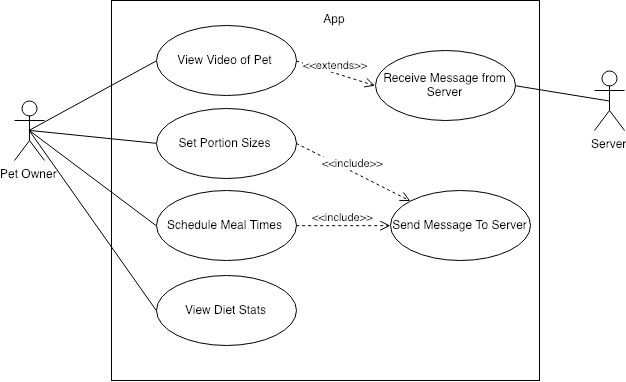
\includegraphics[width=14cm]{UseCaseDiagram.jpg} \\

    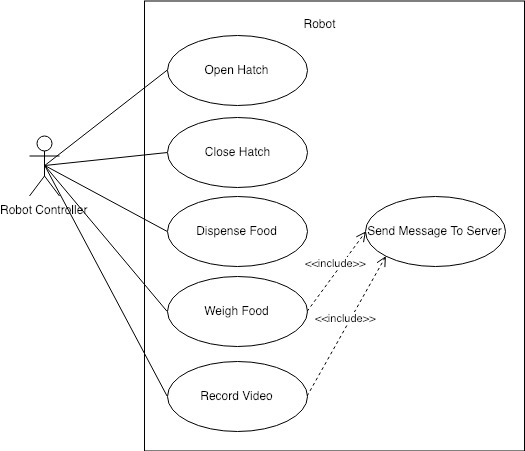
\includegraphics[width=14cm]{UseCaseDiagram1.jpg}
    
    
    \subsection{Software Specifications}
        \subsubsection{App}
        The app will be built as a web app (runs in the browser) using React.js. We decided to build a web app over a native app as web apps require no installation and updates can be pushed without user interaction. It also allows the user to access the app via a mobile phone browser, or a desktop browser. We will be using the React.js framework to build the web app as it allows us to take a modular component based approach to development. This will make our code more clean and maintainable, and increase development speed in the long run.

        
        \subsubsection{Server}
        The server will serve many functions in this project. As well as a REST api for user data, it will have to serve as a message broker between the app and the robot. Further down the timeline it will have to serve as a streaming service for video. Due to the many functions the server will have to provide, we have chosen the Spring framework as the main technology to be used for this part of the project. Spring Boot allows us to painlessly set up message brokers and RESTful API’s faster than most other web frameworks would allow. 


    \subsection{Milestones}
        \subsubsection{Demo 1}
        \begin{itemize}
            \setlength{\itemindent}{.2in}
            \item Robot can dispense food into a bowl (without the weighing chamber)
                \begin{itemize}
                \setlength{\itemindent}{.3in}
                    \item Need 2 hatches to open and drop food into the chute which goes towards the bowl
                \end{itemize}
            \item App has homepage, login and sign up pages 
                \begin{itemize}
                    \setlength{\itemindent}{.3in}
                    \item Allows pet owners to create an account and sign in so they can use the robot 
                \end{itemize}
            \item Server has user authentication
                \begin{itemize}
                    \setlength{\itemindent}{.3in}
                    \item Makes sure that only authorized users have access to the app and the robot 
                \end{itemize}
            \item Server can send and receive messages from the app and the robot
                \begin{itemize}
                    \setlength{\itemindent}{.3in}
                    \item Allows the app and the robot to communicate 
                \end{itemize}
        \end{itemize}
        \subsubsection{Demo 2}
        \begin{itemize}
        \setlength{\itemindent}{.2in}
            \item Robot can rotate such that it can dispense the food into the specified bowl 
                \begin{itemize} 
                    \setlength{\itemindent}{.3in}
                    \item Makes sure the right pet with the associated food is fed 
                \end{itemize}
            \item Robot will dispense the food at a specified time
                \begin{itemize}
                    \setlength{\itemindent}{.3in}
                    \item Checks that the scheduler works 
                \end{itemize}
            \item The bowls have been 3D printed
                \begin{itemize}
                    \setlength{\itemindent}{.3in}
                    \item Allows us to put weight sensors in the bowls
                \end{itemize}
            \item Camera is mounted on the robot
                \begin{itemize}
                    \setlength{\itemindent}{.3in}
                    \item Means that we can make the camera rotate
                \end{itemize}
            \item Server can store and execute a plan
                \begin{itemize}
                    \setlength{\itemindent}{.3in}
                    \item Sends the time the owners wants the pet to be fed from the app to the robot
                \end{itemize}
            \item App has a scheduler
                \begin{itemize}
                    \setlength{\itemindent}{.3in}
                    \item Allows users to create a time for the robot to feed their pet
                \end{itemize}
            \item App can send plans to the server
                \begin{itemize}
                    \setlength{\itemindent}{.3in}
                    \item Sends that specific time to the server 
                \end{itemize}
        \end{itemize}
        \subsubsection{Demo 3}
            \begin{itemize}
                \setlength{\itemindent}{.2in}
                \item Camera can record video
                    \begin{itemize}
                        \setlength{\itemindent}{.3in}
                        \item Allows the robot to send the video to the server
                    \end{itemize}
                \item Set up Bluetooth chips
                    \begin{itemize}
                        \setlength{\itemindent}{.3in}
                        \item Allows us to know where the pets are 
                    \end{itemize}
                \item Server can process video and send to app
                    \begin{itemize}
                        \setlength{\itemindent}{.3in}
                        \item Allows the app to have access to the video 
                    \end{itemize}
                \item Camera can rotate
                    \begin{itemize}
                        \setlength{\itemindent}{.3in}
                        \item Means that the user track the pet
                    \end{itemize}
                \item App can play video
                    \begin{itemize}
                        \setlength{\itemindent}{.3in}
                        \item Allows the user to see their pet 
                    \end{itemize}
                \item Bowls can sense how much weight is in them
                    \begin{itemize}
                        \setlength{\itemindent}{.3in}
                        \item Allows us to know how food is in the bowl
                    \end{itemize}
                \item Bowls can send messages to the server
                    \begin{itemize}
                        \setlength{\itemindent}{.3in}
                        \item Allows the robot to distribute the right amount of food
                    \end{itemize}
            \end{itemize}
        \subsubsection{Demo 4}
        \begin{itemize}
            \setlength{\itemindent}{.2in}
            \item Live stream on app
                \begin{itemize}
                    \setlength{\itemindent}{.3in}
                    \item Means that the user can see the pet in real time 
                \end{itemize}
            \item Bowls have flaps that open when the pet is nearby
                \begin{itemize}
                    \setlength{\itemindent}{.3in}
                    \item So the one pet doesn’t eat the other pet’s food
                \end{itemize}
            \item App has pet analytics
                \begin{itemize}
                    \setlength{\itemindent}{.3in}
                    \item Allows the user to track how much food their pets have eaten
                \end{itemize}
        \end{itemize}
        \subsubsection{Extensions}
        \begin{itemize}
        \setlength{\itemindent}{.2in}
            \item Robot has a laser pointer (so it can play with the pet)
                \begin{itemize}
                    \setlength{\itemindent}{.3in}
                    \item Allows the user to play with the pet while they are away
                \end{itemize}
        \end{itemize}